\chapter{Description générale}

\section{Environnement du projet}
Pour ce projet, je me base sur le code de mon encadrant, qui résout le sous-problème où l'ordre de réalisation des jobs et la constitution des lots sont fixés.
Le code est écrit en C++ avec Visual studio 2017 et utilise la bibliothèque Cplex.

Le projet existant utilise des fonctionnalités de Visual c++ et n'est pas compatible avec le C++ standard,
 une partie de mon travail consiste à l'adapter.
\section{Caractéristiques des utilisateurs}
Il s'agit d'un projet de recherche, les utilisateurs seront des chercheurs souhaitant tester les algorithmes développés dans ce projet.
 
\section{Fonctionnalités du système}
L'application développée dans ce projet a pour objectif de trouver la meilleure solution pour le problème défini précédemment.
Elle est utilisée pour comparer les résultats des différents algorithmes.
Deux méthodes sont explorées, une méthode exacte utilisant un solveur et l'autre une méthode heuristique.

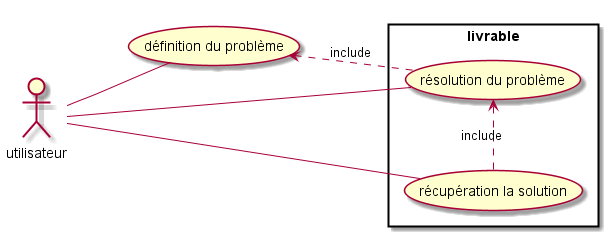
\includegraphics[width=\textwidth]{parts/description_generale/use_cases}
\section{Structure générale du système}

Le programme comprendra une partie commune pour les deux algorithmes.
Cette partie commune comprendra :
\begin{itemize}
    \item les descriptions des instances.
    \item les descriptions des solutions.
    \item les validations des solutions.
\end{itemize}

L'utilisateur pourra choisir la méthode a utiliser.